\subsection*{Цель работы}

\begin{enumerate}
    \item Изучить устройство и технические характеристики устройства управления ``Сфера-36'' и промышленного робота PM-01.
    \item Изучить порядок включения и калибровки робота.
\end{enumerate}

\subsection*{Выполнение}

Технические характеристики манипулятора отображены в таблице~\ref{tab:tech}. Степени подвижности ПР PM-01 показаны на рисунке~\ref{fig:moves}. Технические характеристики УУ ``Сфера-36'' отображены в таблице~\ref{tab:sphere}.

Структурные схемы УУ ``Сфера-36'' и следящего привода одного звена приведены на рисунках~\ref{fig:str1},~\ref{fig:str2} приложения А.

\begin{longtable}[c]{|c|C{9cm}|C{5cm}|}
\caption{Технические характеристики манипулятора PM-01\label{tab:tech}}\\
\hline
\textbf{№} & \textbf{Параметр} & \textbf{Значение}\\
\hline
\endfirsthead
\hline
\textbf{№} & \textbf{Параметр} & \textbf{Значение}\\
\hline
\endhead
		1 & Номинальная грузоподъемность, кг & 2,5 \\
        \hline
        2 & Максимальная погрешность позиционирования, мм, не более & $\pm$ 0,1 \\
        \hline
        3 & Максимальная скорость перемещения, м/с, не менее & 0,5 \\
        \hline
        4 & Диапазон поворотов по степени подвижности, град, не менее & \\
        & степень 1 & 320\\
        & степень 2 & 266\\
        & степень 3 & 284\\
        & степень 4 & 280\\
        & степень 5 & 200\\
        & степень 6 & 520\\
        \hline
        5 & Тип привода & электрический постоянного тока\\
        \hline
        6 & Число одновременно управляемых движений по степеням подвижности & 6\\
        \hline
        7 & Напряжение питания, В & однофазное 220\\
        \hline
        8 & Потребляемая мощность, Вт, не более & 1200\\
        \hline
        9 & Масса, кг, не более & 62\\
        \hline
        10 & Наработка робота на отказ, ч & 500\\
        \hline
        11 & Средний срок службы, лет, не менее & 10\\
        \hline
        12 & Радиус рабочей зоны манипулятора, м & 0,864\\
        \hline
\end{longtable}

\begin{figure}[ht]
\centering
    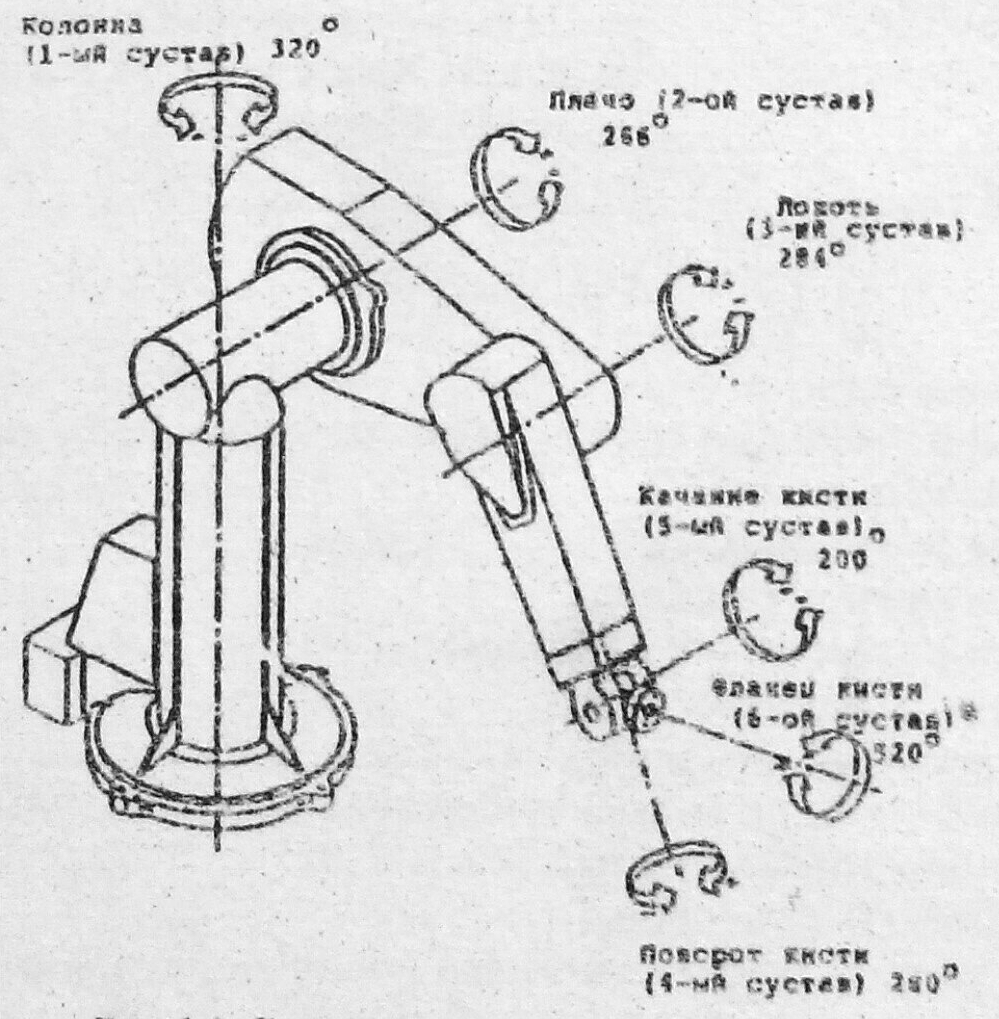
\includegraphics[scale=0.3]{Figures/1.png}
    \caption{Степени подвижности манипулятора\label{fig:moves}}
\end{figure}

\begin{longtable}[c]{|C{5cm}|C{9cm}|}
\caption{Технические характеристики УУ ``Сфера-36''\label{tab:sphere}}\\
		\hline
        Принцип управления & двухуровневое микропроцессорное\\
        \hline
        Язык программирования & ARPS\\
        \hline
        Устройства обучения и программирования & дисплей с клавиатурой и пульт ручного управления\\
        \hline
        ОЗУ пользователя & умкость: 8 килослов, с произвольным доступом и резервным питанием от аккумулятора\\
        \hline
        Внешнее ЗУ & НГМД, емкость 33,8 К слов\\
        \hline
        Входы и выходы & по 32 дискретных входа и выхода\\
        & входы: 24 В пост. тока, 15 МА\\
        & выходы: 24 В пост. тока, 2 А\\
        \hline
        Масса, кг & 280\\
        \hline
\end{longtable}

\subsection*{Условные обозначения}

\subsubsection*{Верхний уровень}

\begin{itemize}
    \item МЦП - модуль центрального процессора;
    \item ОЗУ - оперативное запоминающее устройство;
    \item ПЗУ - постоянное запоминающее устройство;
    \item МПИ - модуль последовательного интерфейса;
    \item МАВ - модуль аналогового ввода;
    \item МВВ - модуль ввода-вывода;
    \item МС - модуль связи М1 и М2.
\end{itemize}

\subsubsection*{Нижний уровень}

\begin{itemize}
    \item МПП - модуль процессора привода;
    \item МУП - модуль управления приводом;
    \item ШИП - широтно-импульсный преобразователь.
\end{itemize}

\subsubsection*{Следящий электропривод звена манипулятора}
\begin{itemize}
    \item ФИД - фотоимпульсный датчик;
    \item ФПИ - формирователь позиционных импульсов;
    \item ГИ - генератор импульсов;
    \item ДВИ - датчик временного интервала;
    \item ДПП - датчик переменных позиций;
    \item РДВИ - регистр длительности временного интервала;
    \item РДПП - регистр длительности приращения позиции;
    \item ПКШИ - преобразователь кода управления в широтно-модулированный сигнал;
    \item ДТ - датчик тока.
\end{itemize}

\subsubsection*{Магистрали}

\begin{itemize}
    \item М1 - магистраль центрального процессора;
    \item M2 - магистраль процессоров приводов.

\end{itemize}

\subsection*{Выводы}

Мультипроцессорная система управления ``Сфера-36'' состоит из верхнего и нижнего уровней, позволяя эффективно решать задачи управления манипулятором в реальном времени. Верхний уровень занимается расчетом точек и траекторий (интерполяцией), обработкой и обменом дискретными сигналами с различными устройствами, а также предоставляет возможность диалога с оператором и возможность ручного управления манипулятором от ПРУ, в то время как нижний уровень управляет непосредственно приводами на основе программ верхнего уровня.

В лабораторной работе мы разобрались с внутренним устройством и структурой СУ ``Сфера-36''и познакомились с назначением основных модулей УУ.

\clearpage

\subsection*{Приложение А}

\begin{figure}[ht]
\centering
    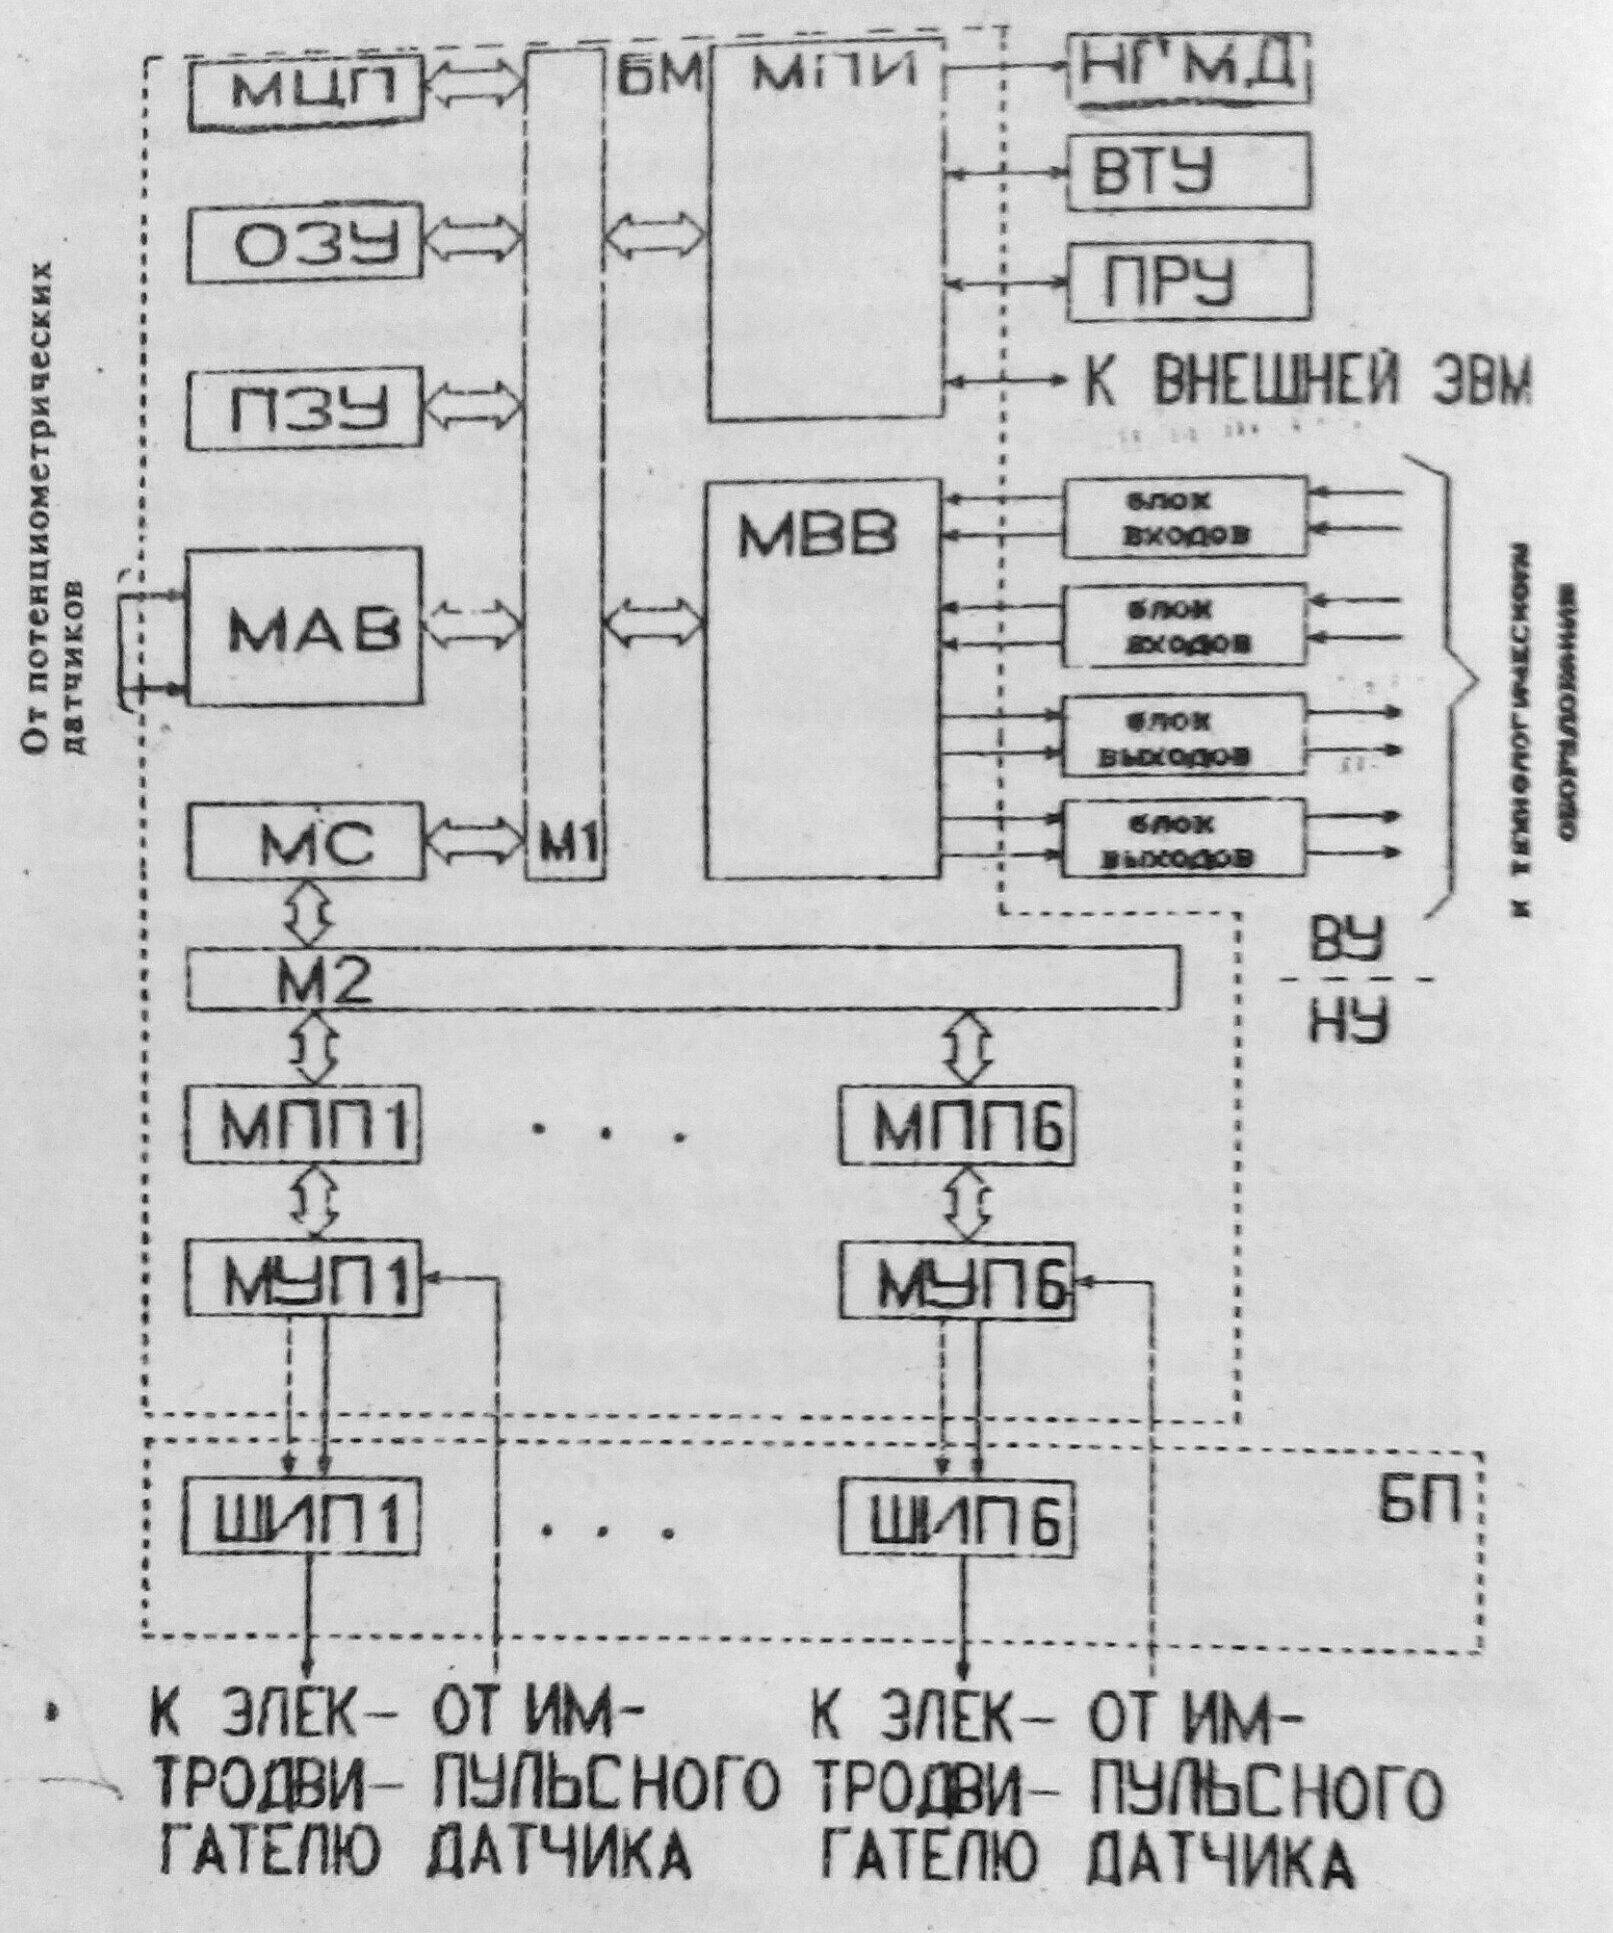
\includegraphics[scale=0.25]{Figures/2.png}
    \caption{Структурная схема УУ ``Сфера-36''\label{fig:str1}}
\end{figure}

\begin{figure}[ht]
\centering
    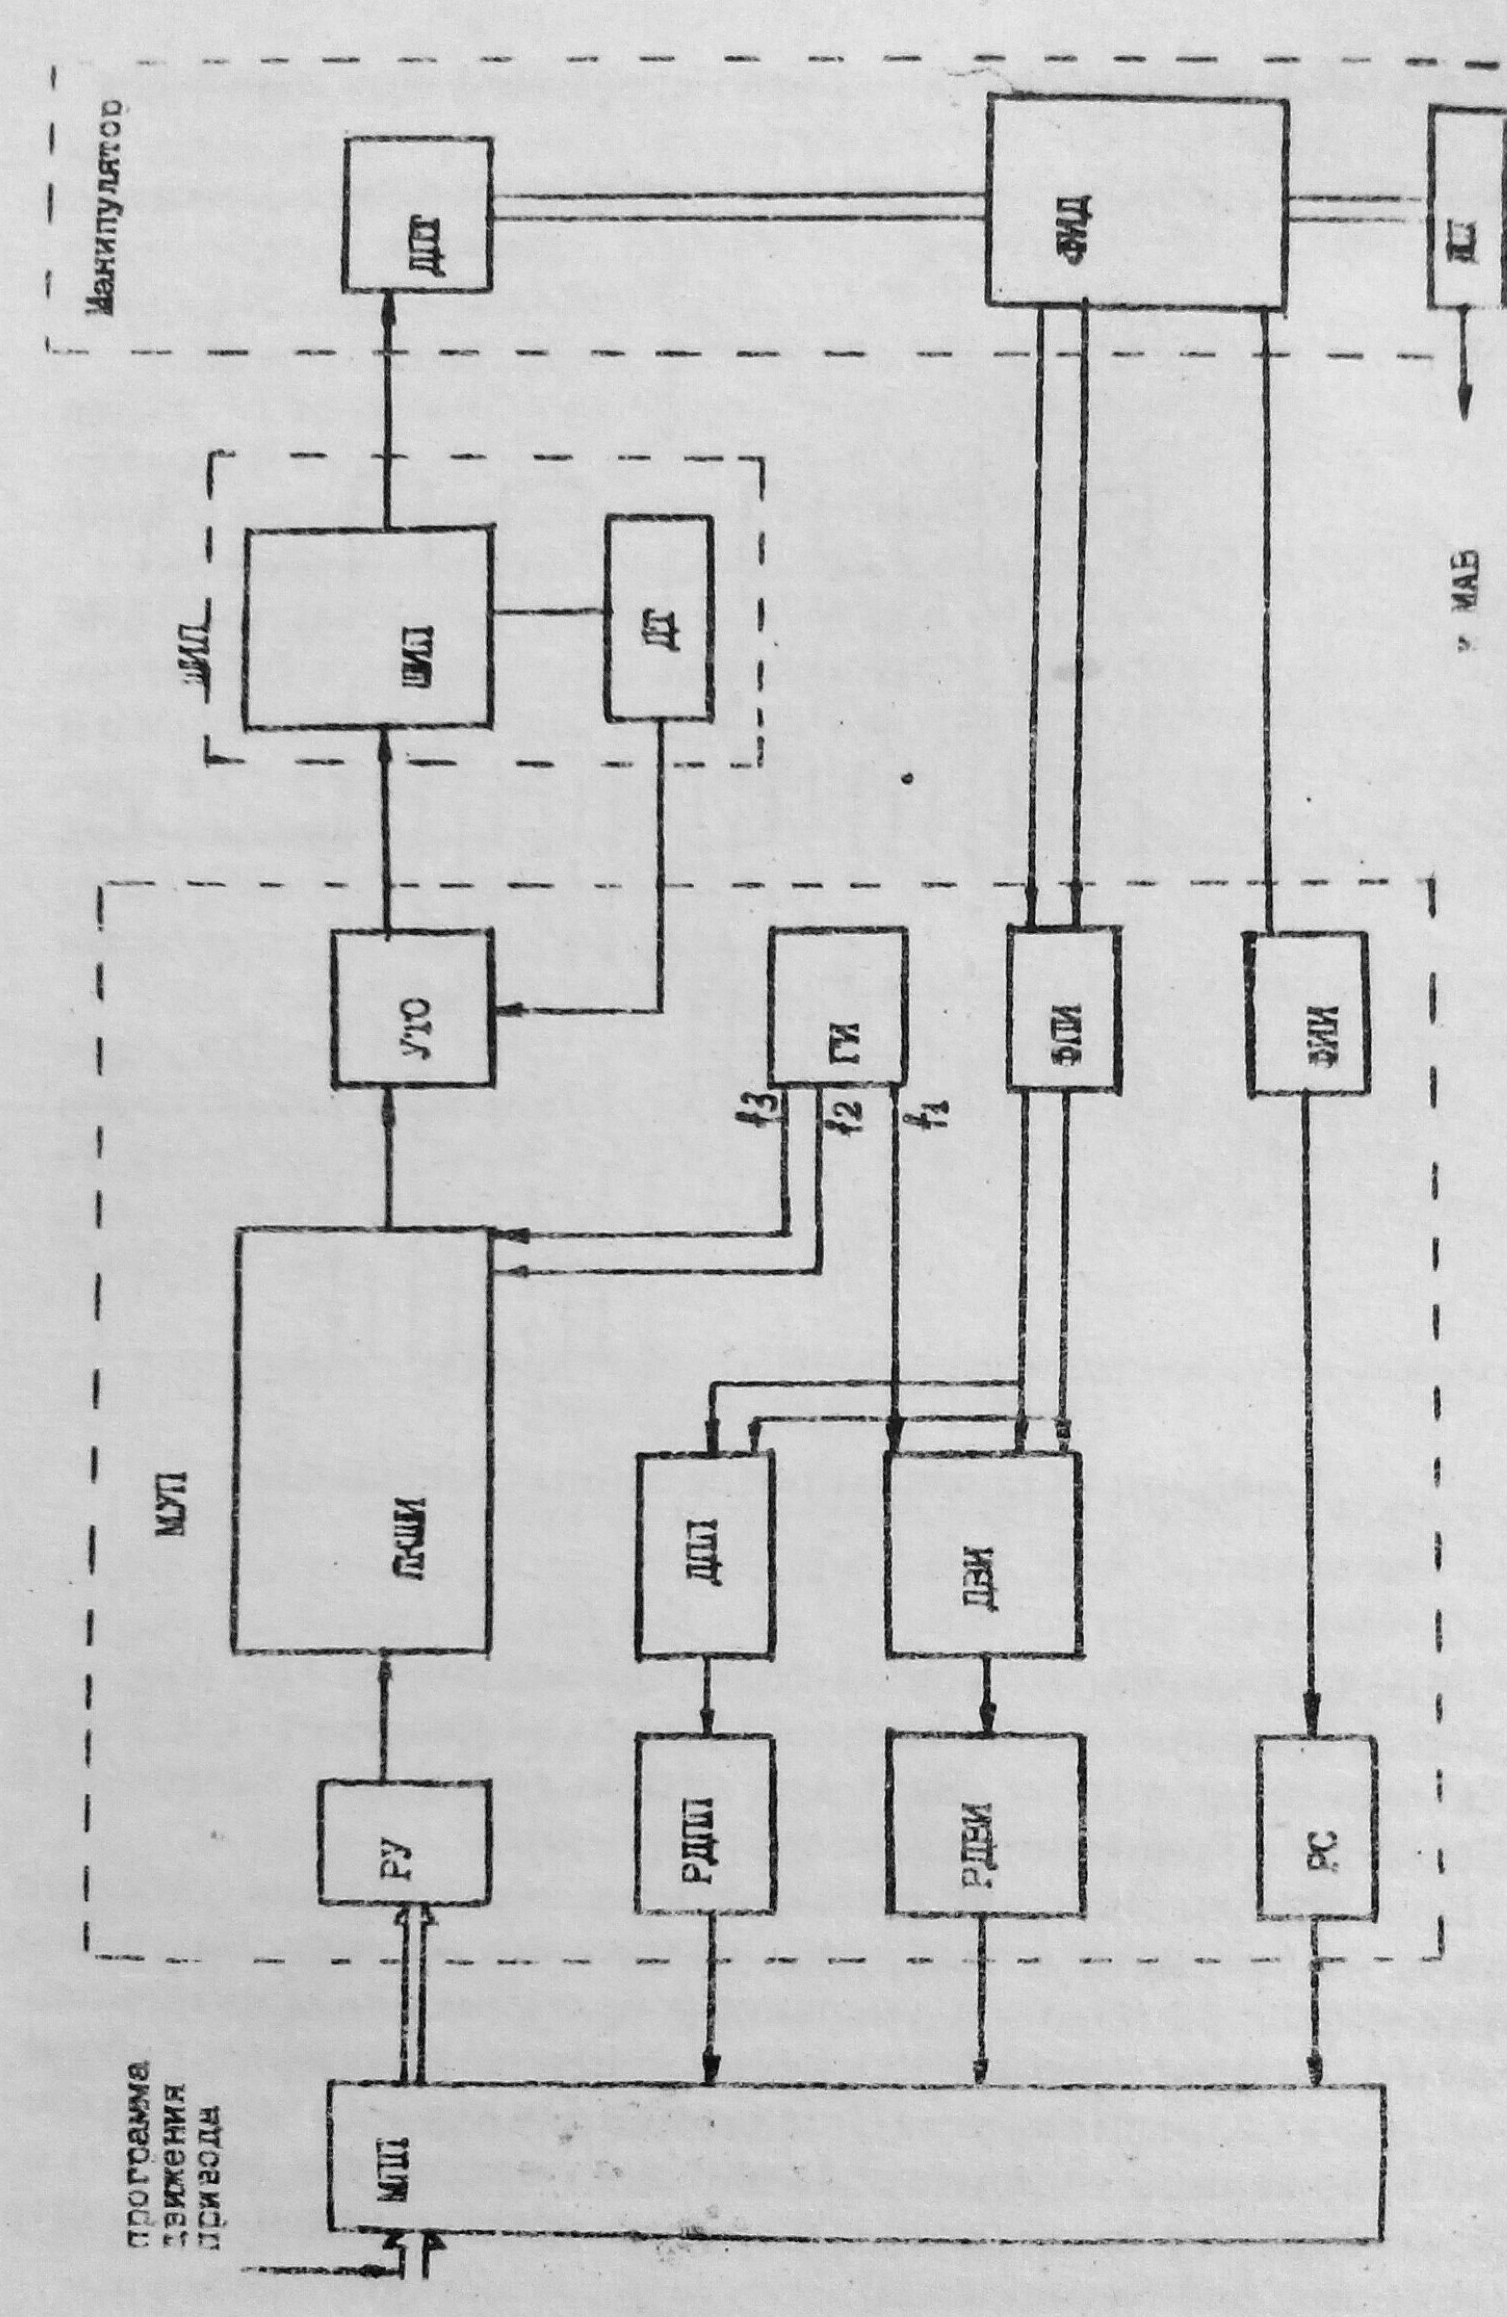
\includegraphics[scale=0.25]{Figures/3.png}
    \caption{Структурная схема следящего электропривода одного звена\label{fig:str2}}
\end{figure}

\clearpage
